\documentclass[a4paper]{article}

%%%%%%%% CREATE DOCUMENT STRUCTURE %%%%%%%%
%% Language and font encodings
\usepackage[english]{babel}
\usepackage[utf8x]{inputenc}
\usepackage[T1]{fontenc}
%\usepackage{subfig}

%% Sets page size and margins
\usepackage[a4paper,top=3cm,bottom=2cm,left=2cm,right=2cm,marginparwidth=1.75cm]{geometry}

%% Useful packages
\usepackage{amsmath}
\usepackage{graphicx}
\usepackage[colorinlistoftodos]{todonotes}
\usepackage[colorlinks=true, allcolors=blue]{hyperref}
\usepackage{caption}
\usepackage{subcaption}
\usepackage{sectsty}
\usepackage{apacite}
\usepackage{float}
\usepackage{titling} 
\usepackage{blindtext}
\usepackage[square,sort,comma,numbers]{natbib}
\usepackage[colorinlistoftodos]{todonotes}
\usepackage{xcolor}
\definecolor{darkgreen}{rgb}{0.0, 0.4, 0.0}

%%%%%%%% DOCUMENT %%%%%%%%
\setlength {\marginparwidth }{2cm}
\begin{document}

%%%% Title Page
\begin{titlepage}

\newcommand{\HRule}{\rule{\linewidth}{0.5mm}} 							% horizontal line and its thickness
\center 
 
% University
\textsc{\LARGE BRAC UNIVERSITY }\\[1cm]

% Document info
\textsc{\Large \textbf{MAT 110}}\\[0.2cm] 										% Course Code
\HRule \\[0.4cm]
{ \huge \bfseries MATH I \\[0.4cm]Differential Calculus and Co-ordinate Geometry}\\[0.7cm]								% Assignment
\HRule \\[2cm]
\Large
{NAME : \textsc{\textbf{TANAY PAUL}}}\\
ID : \textbf{21301438}\\[1.5cm]
% Author 

\includegraphics[width=0.4\textwidth]{images/bracu_logo.png}\\[0.4cm] 	% University logo
\vfill 
\newpage
\section*{}
\begin{figure}[h]
    \centering
    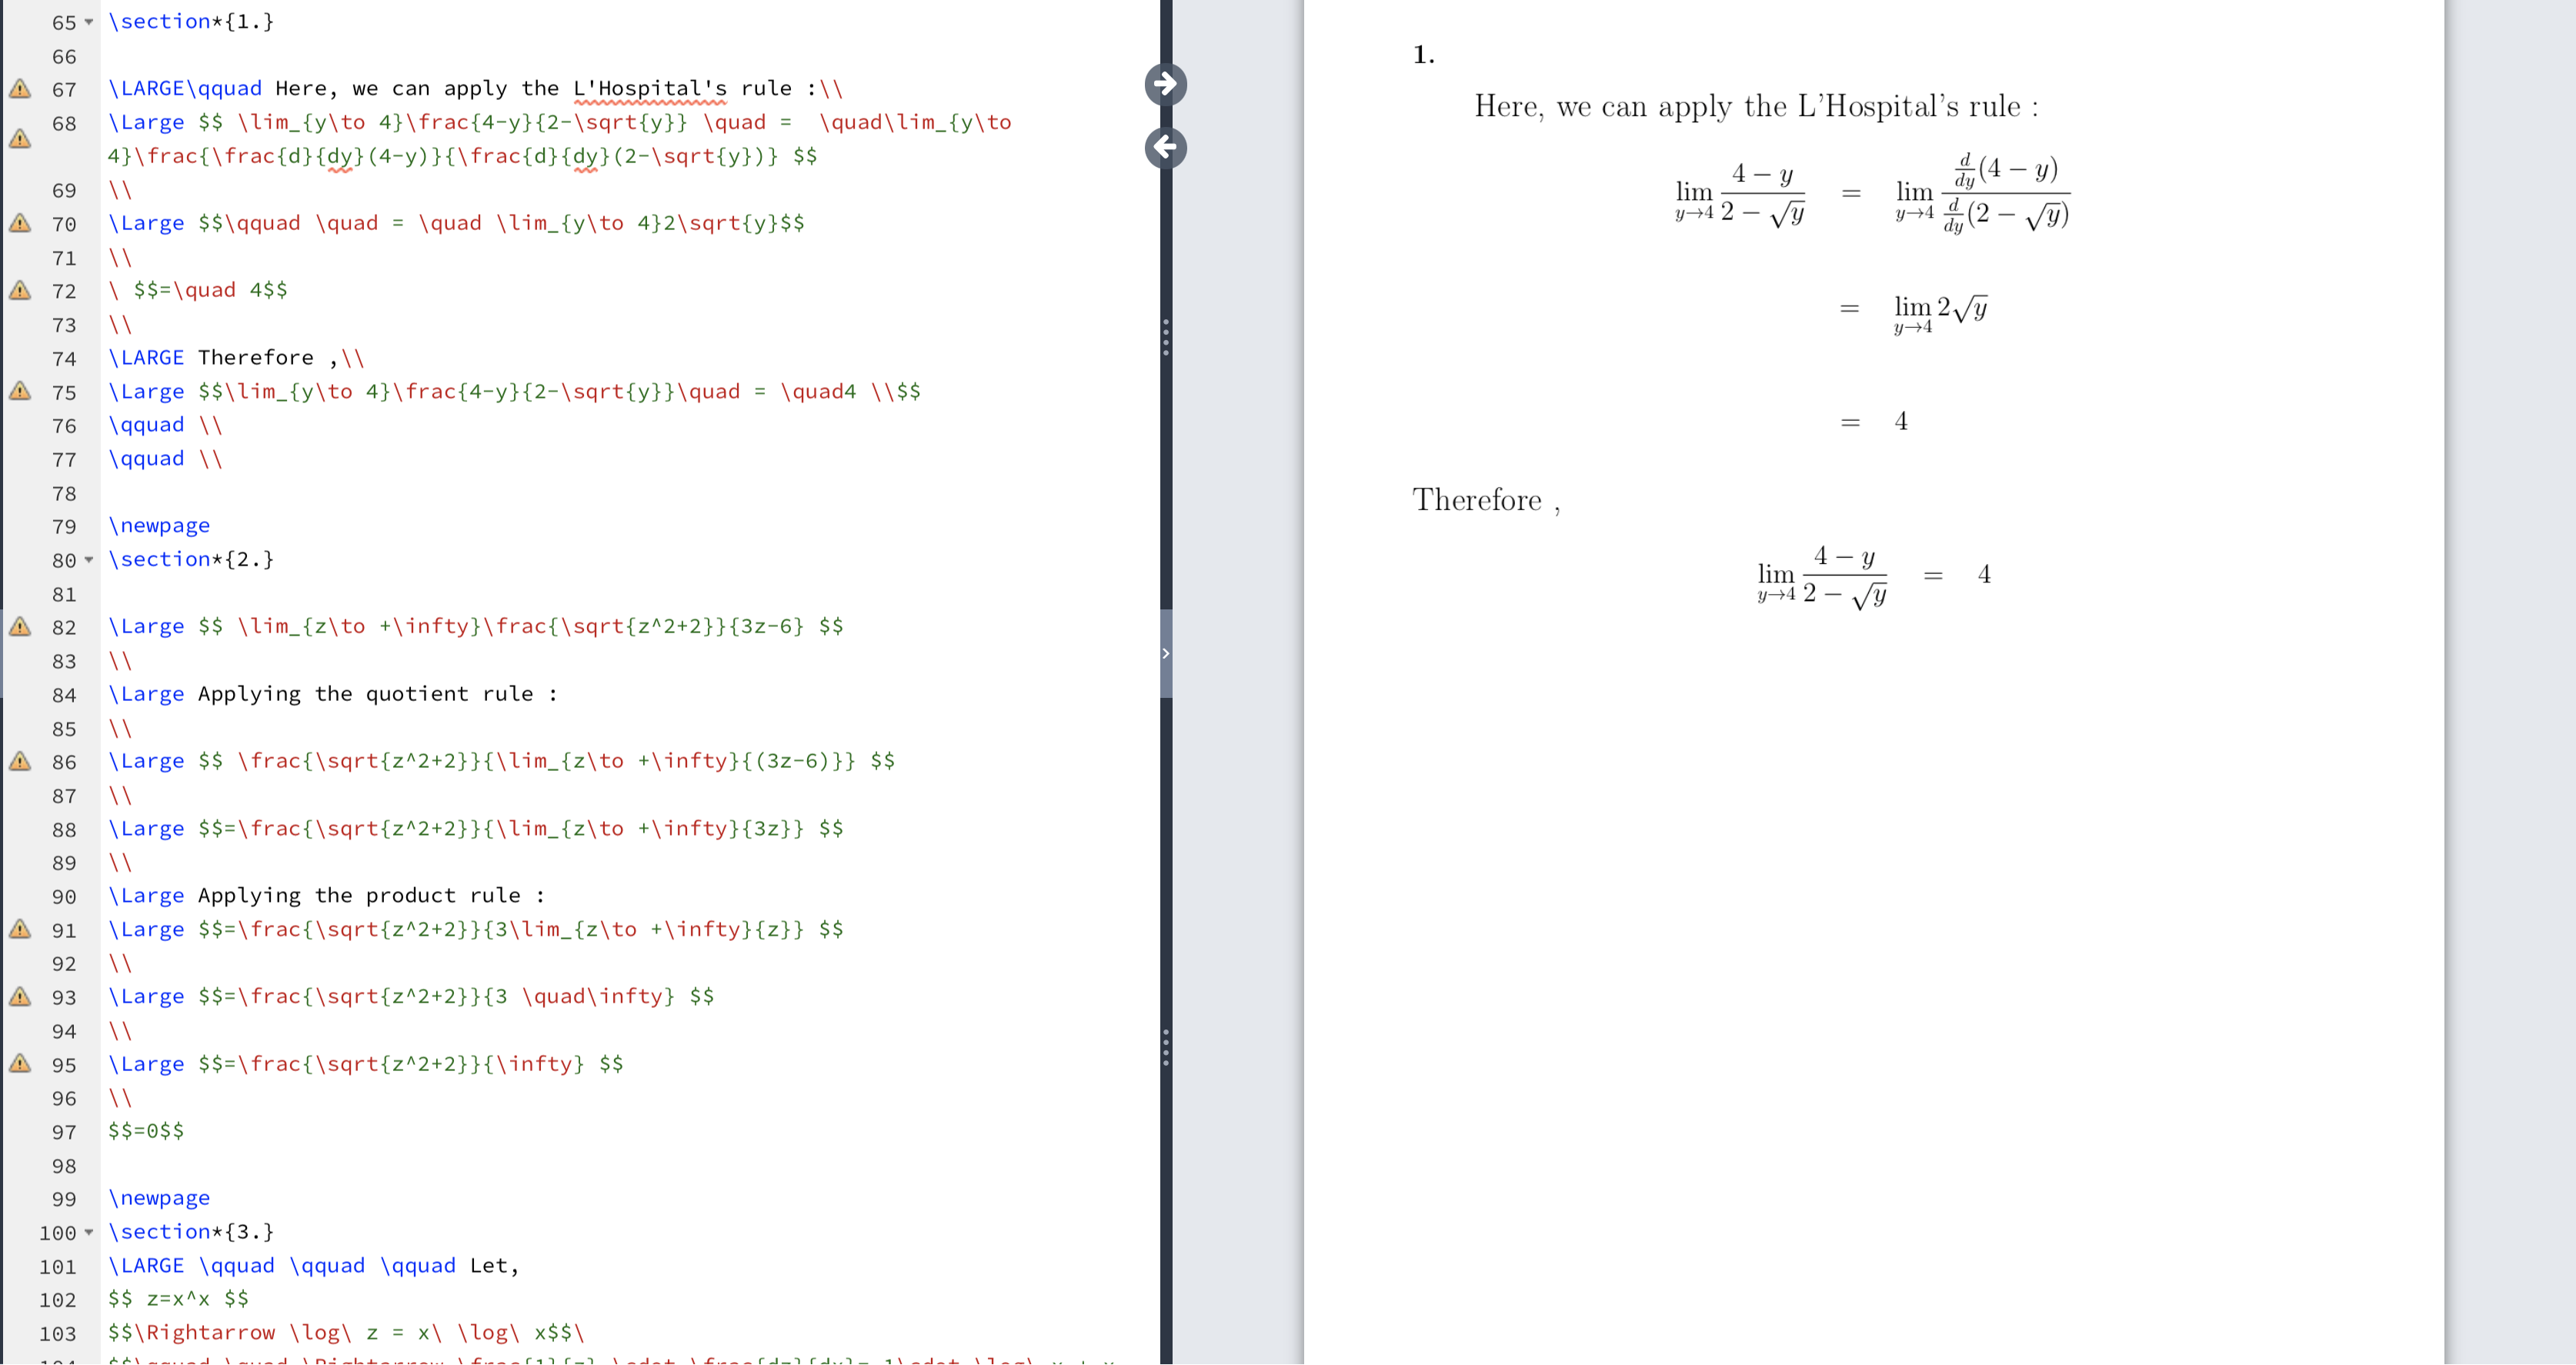
\includegraphics[scale=0.3]{ss.png}
    \caption{Latex Screenshot }
    \label{fig:my_label}
\end{figure}
\end{titlepage}

%%%% SECTIONS
%% Section 1

\section*{1.}

\LARGE\qquad Here, we can apply the L'Hospital's rule :\\
\Large $$ \lim_{y\to 4}\frac{4-y}{2-\sqrt{y}} \quad =  \quad\lim_{y\to 4}\frac{\frac{d}{dy}(4-y)}{\frac{d}{dy}(2-\sqrt{y})} $$
\\
\Large $$\qquad \quad = \quad \lim_{y\to 4}2\sqrt{y}$$
\\
\ $$=\quad 4$$
\\
\LARGE Therefore ,\\
\Large $$\lim_{y\to 4}\frac{4-y}{2-\sqrt{y}}\quad = \quad4 \\$$ 
\qquad \\
\qquad \\

\newpage
\section*{2.}

\Large $$ \lim_{z\to +\infty}\frac{\sqrt{z^2+2}}{3z-6} $$
\\
\Large Applying the quotient rule :
\\
\Large $$ \frac{\sqrt{z^2+2}}{\lim_{z\to +\infty}{(3z-6)}} $$
\\
\Large $$=\frac{\sqrt{z^2+2}}{\lim_{z\to +\infty}{3z}} $$
\\
\Large Applying the product rule :
\Large $$=\frac{\sqrt{z^2+2}}{3\lim_{z\to +\infty}{z}} $$
\\
\Large $$=\frac{\sqrt{z^2+2}}{3 \quad\infty} $$
\\
\Large $$=\frac{\sqrt{z^2+2}}{\infty} $$
\\
$$=0$$

\newpage
\section*{3.}
\LARGE \qquad \qquad \qquad Let,
$$ z=x^x $$
$$\Rightarrow \log\ z = x\ \log\ x$$\
$$\qquad \quad \Rightarrow \frac{1}{z} \cdot \frac{dz}{dx}= 1\cdot \log\ x + x \cdot \frac{1}{x}$$\
$$\quad \quad \Rightarrow \frac{dz}{dx} = x^x( 1+\log \ x)$$
\\
$$\qquad y= x^{x^x}= x^z$$
$$\Rightarrow \log \ y = z \cdot \log x$$\
$$ \qquad \qquad \Rightarrow \frac{1}{y} \cdot \frac{dy}{dx} = \frac{dz}{dx}\cdot \log x + z \cdot \frac{1}{x}$$\
$$ \qquad\qquad\qquad\qquad\qquad\qquad = x^x (1+\log x)\cdot \log x + \frac{x^x}{x}$$\
$$ \quad \quad \qquad\qquad\qquad\qquad\qquad\qquad = x^x (1+\log x) \cdot \log x + x^x -1 $$\
$$ \qquad\qquad\quad\qquad\qquad\quad \dot{.\hspace{.095in}.}\hspace{.5in} \frac{dy}{dx} = x^{x^x} \Big[x^x(1+ \log x)\cdot \log x + x^x-1 \Big]$$

\newpage
\section*{4.}
$$\Large \quad x=a $$\\
$$ \lim_{x\to a^-} f'(x) = \lim_{x\to a^+} f'(x) $$\\ \LARGE\qquad\qquad $ x=0 $
$$ \lim_{x\to 0^-} f'(x) = 0 $$\\
$$ \lim_{x\to 0^+} f'(x) = \lim_{x\to 0^+} \cos x = 1$$\\
$$ \lim_{x\to 0^-} f'(x) \neq  \lim_{x\to 0^+} f'(x) $$\\
\LARGE Answer: Function is not Differentiable.
\newpage
\section*{5.}
$$\Large \frac{d}{dx}\ln \Big(\cos{\big(x \big)}\sin{\big(x \big)}\Big)$$
\\
$$ = \ln \Big(\cos{\big(x \big)}\Big) \bigg\{ \frac{d}{dx} \sin{\big(x \big)}\bigg\} + \sin{\big(x \big)} \bigg\{ \frac{d}{dx} \Big( \ln \cos {\big(x \big)}\Big)\bigg\} $$
\\
$$ = \ln \Big(\cos{\big(x \big)}\Big) \cos{\big(x \big)} + \sin{\big(x \big)} \bigg\{ \frac{1}{\cos\big( x \big)} \Big( \- \sin \big( x \big) \Big) \bigg\} $$
\\
$$ = \frac{\ln \Big(\cos{\big(x \big)}\Big) \Big( \cos{^2}{\big(x \big)} - \sin{^2}{\big(x \big)}\Big)}{\cos{\big(x \big)}}$$

\newpage
\section*{6.}
$$ \Large y = x^2 (\sin{^-{^1}}x)^3 $$
\\
$$ \Large \frac{dy}{dx} = x^2\cdot 3 \bigg\{(\sin{x})^-{^1}\bigg\}^2 \cdot \frac{1}{\sqrt{1-x^2}} + 2x \cdot \bigg\{(\sin{x})^-{^1}\bigg\}^3 $$
\\
$$\Large \frac{dy}{dx} = \frac{3x^2\bigg\{(\sin{x})^-{^1}\bigg\}^2}{\sqrt{1-x^2}} + 2x \bigg\{(\sin{x})^-{^1}\bigg\}^3 $$

\end{document}